\documentclass[12pt,crop]{standalone}
\usepackage{fontspec}
\usepackage{libertinus}
\usepackage{xcolor}
\usepackage{tikz}
\usetikzlibrary{automata,arrows.meta,fadings,positioning}

\definecolor{state-border-color}{HTML}{457b9d}
\definecolor{final-state-fill-color}{HTML}{A8DADC}
\definecolor{state-text-color}{HTML}{1D3557}
\definecolor{trans-text-color}{HTML}{05668D}

\begin{document}
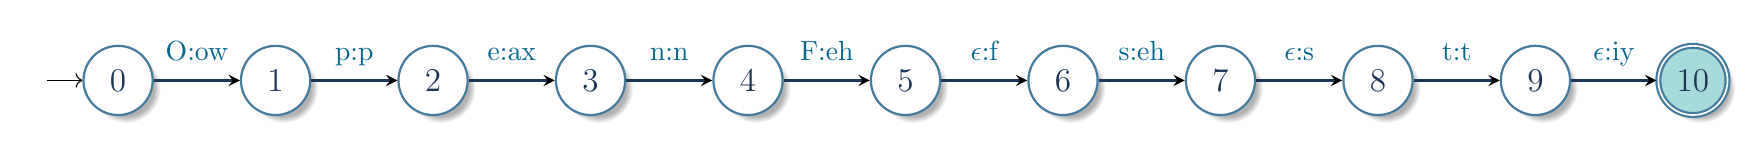
\begin{tikzpicture}[
    node distance = 2cm,
    on grid,
    auto,
    every state/.style = {
      circle,
      thick,
      fill=white,
      draw=state-border-color,
      text=state-text-color,
      font={\bfseries\large#1},
      preaction={
        fill=black,opacity=.3,
        path fading=circle with fuzzy edge 20 percent,
        transform canvas={xshift=1mm,yshift=-1mm}
      }
    },
    every node/.style = {
      text=trans-text-color
    }
  ]
  % States.
  \node (s0) [state, initial, initial text = {}] {$0$};
  \node (s1) [state, right of = s0] {$1$};
  \node (s2) [state, right of = s1] {$2$};
  \node (s3) [state, right of = s2] {$3$};
  \node (s4) [state, right of = s3] {$4$};
  \node (s5) [state, right of = s4] {$5$};
  \node (s6) [state, right of = s5] {$6$};
  \node (s7) [state, right of = s6] {$7$};
  \node (s8) [state, right of = s7] {$8$};
  \node (s9) [state, right of = s8] {$9$};
  \node (s10) [state, accepting, right of = s9, fill=final-state-fill-color] {$10$};

  % Transitions.
  \path [-stealth, thick, draw=state-text-color]
  (s0) edge node {O:ow\strut} (s1)
  (s1) edge node {p:p\strut} (s2)
  (s2) edge node {e:ax\strut} (s3)
  (s3) edge node {n:n\strut} (s4)
  (s4) edge node {F:eh\strut} (s5)
  (s5) edge node {$\epsilon$:f\strut} (s6)
  (s6) edge node {s:eh\strut} (s7)
  (s7) edge node {$\epsilon$:s\strut} (s8)
  (s8) edge node {t:t\strut} (s9)
  (s9) edge node {$\epsilon$:iy\strut} (s10);
\end{tikzpicture}
\end{document}
